\subsection{Processo per la generazione di allerte temporale}

\subparagraph{Legenda (figura \ref{Allerta_temporale}):}
\begin{itemize}
	\item $T = $ \{insieme \textit{datetime}, ossia data + orario\};
	\item $t \in A = \{x, t_0, t_f \in T, n \in \mathbb{N}| x = t_0 + n \cdot T_{up} \cup x \leq t_f\}$ con:
	\begin{itemize}
		\item $t_0$ = istante temporale 24 ore precedente l'ultima rilevazione di pressione atmosferica $p_{atm}(t_f)$;
		\item $t_f$ = istante temporale relativo all'ultima rilevazione di pressione atmosferica $p_{atm}(t_f)$;   
		\item $T_{up}$ = intervallo temporale che intercorre tra due rilevazioni consecutive svolte dalla stazione meteorologica d'interesse, in genere \SI{10}{\minute}.  
	\end{itemize}
	\item $I_1 \subset A = $ \{sottoinsieme di A contenente gli istanti temporali relativi alle prime 2 rilevazioni di $p_{atm}(t)$ a partire dall'istante 3 ore precedente $t_f$\};
	\item $I_2 \subset A = $ \{sottoinsieme di A contenente gli istanti temporali relativi alle ultime 2 rilevazioni di $p_{atm}(t)$\};
	\item $p^{mean}_{low} = \frac{1}{2} \cdot \sum_{i = 1}^{I_1} p_{atm}(i)$;
	\item $p^{mean}_{up} = \frac{1}{2} \cdot \sum_{i = 1}^{I_2} p_{atm}(i)$;
	\item $\Delta_{old}$ = variazione di pressione atmosferica relativa alla precedente esecuzione dell'algoritmo;
	\item $t_{f, old}$ = istante temporale relativo all'ultima rilevazione di pressione atmosferica con riferimento alla precedente esecuzione dell'algoritmo;
	\item $t_r$ = istante temporale in cui è stata eseguita dalla stazione meteorologica d'interesse l'ultima rilevazione di pressione atmosferica presente nel database. 
\end{itemize}

\begin{figure}[h!]
	\centering
	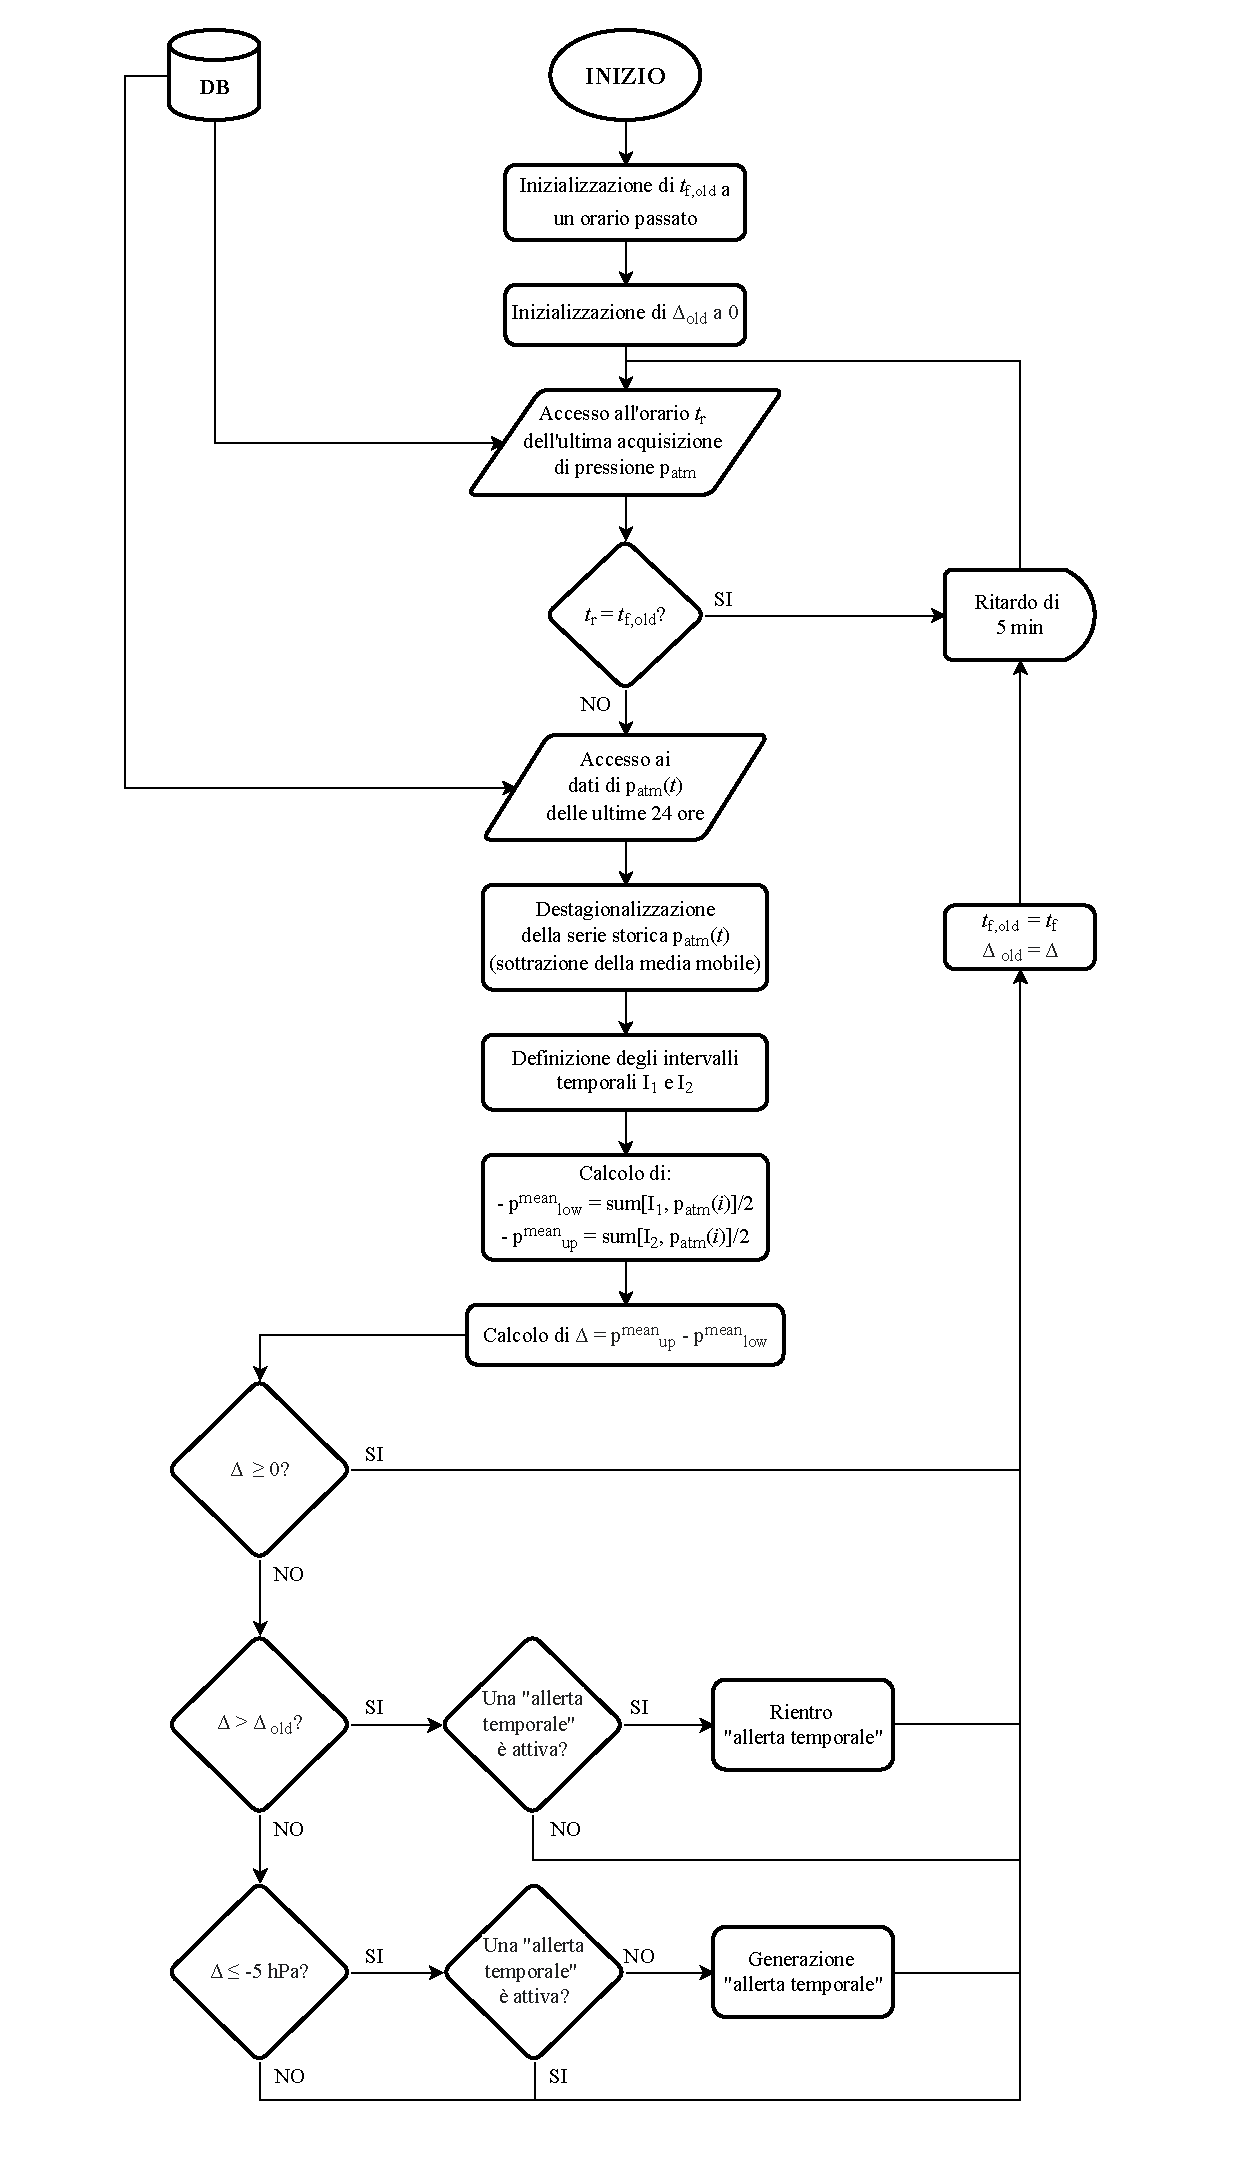
\includegraphics[height=580px]{FlowChartsFiles/Allerta_temporale.pdf}
	\caption[Diagramma di flusso relativo al processo di generazione di allerte temporale]{diagramma di flusso relativo al processo di generazione di allerte temporale.}
	\label{Allerta_temporale}
\end{figure}

\subsection{Processo per la generazione di allerte nebbia e brina}

\subparagraph{Legenda (figure \ref{Allerta_nebbia_&_brina_1} e \ref{Allerta_nebbia_&_brina_2}):}
\begin{itemize}
	\item $T = $ \{insieme \textit{datetime}, ossia data + orario\};
	\item $t \in A = \{x, t_0, t_f \in T, n \in \mathbb{N}| x = t_0 + n \cdot T_{up} \cup x \leq t_f\}$ con:
	\begin{itemize}
		\item $t_0$ = istante temporale 24~ore precedente l'ultima rilevazione di pressione atmosferica $p_{atm}(t_f)$;
		\item $t_f$ = istante temporale relativo all'ultima rilevazione di pressione atmosferica $p_{atm}(t_f)$;   
		\item $T_{up}$ = intervallo temporale che intercorre tra due rilevazioni consecutive svolte dalla stazione meteorologica d'interesse, in genere \SI{10}{\minute}.  
	\end{itemize}
	\item $t_1 = t_f + 1 \cdot T_{up}$ = istante temporale a cui viene svolta la predizione a 1~passo; 
	\item $t_2 = t_f + 2 \cdot T_{up}$ = istante temporale a cui viene svolta la predizione a 2~passi;
	\item $t_3 = t_f + 3 \cdot T_{up}$ = istante temporale a cui viene svolta la predizione a 3~passi;
	\item IC$_{1}$ = intervallo di confidenza al \SI{95}{\percent} relativo alla predizione a un 1~passo;
	\item IC$_{2}$ = intervallo di confidenza al \SI{95}{\percent} relativo alla predizione a un 2~passi;
	\item IC$_{3}$ = intervallo di confidenza al \SI{95}{\percent} relativo alla predizione a un 3~passi.
	\item $t_{f, old}$ = istante temporale relativo all'ultima rilevazione di temperatura (e umidità relativa) con riferimento alla precedente esecuzione dell'algoritmo;
\end{itemize}

\begin{figure}[h!]
	\centering
	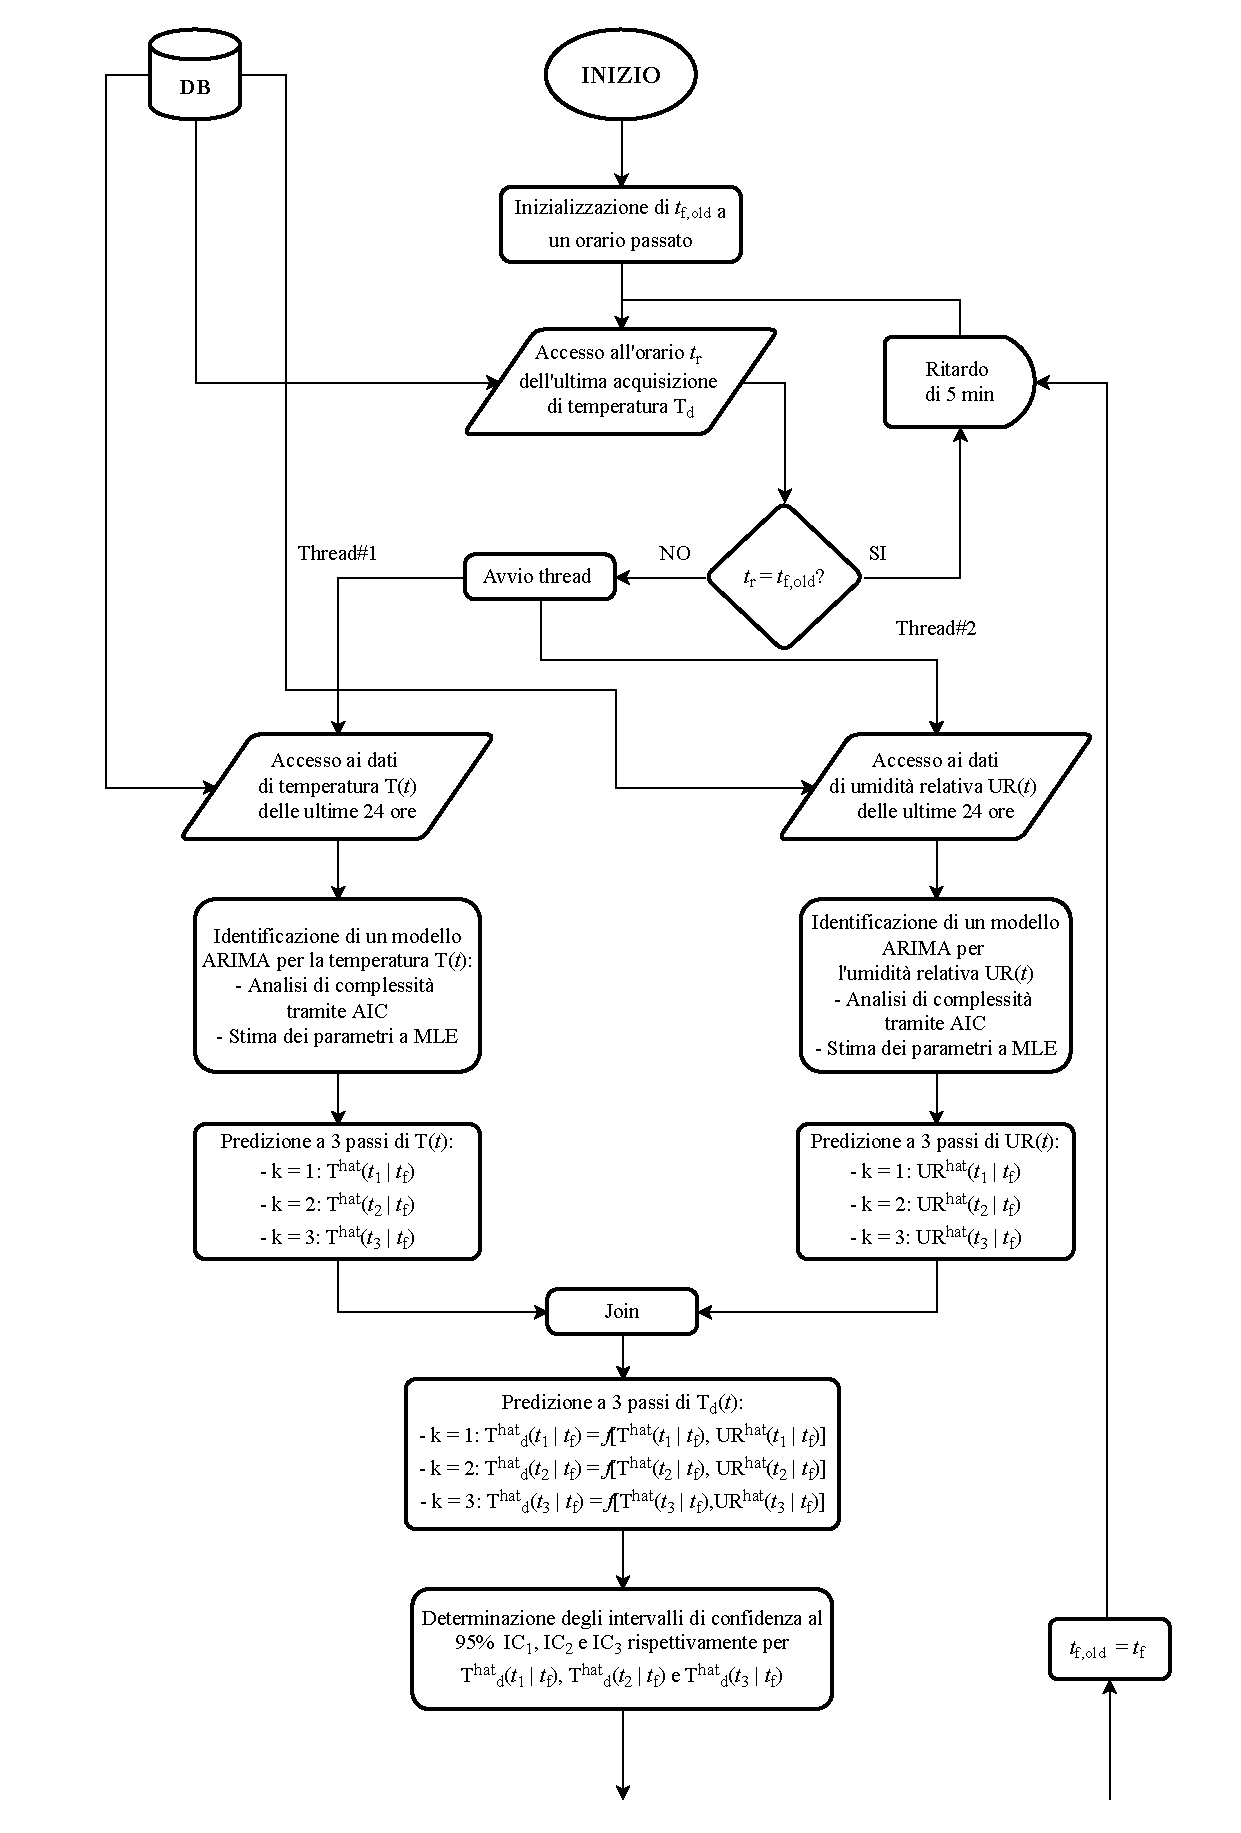
\includegraphics[height=580px]{FlowChartsFiles/Allerte_nebbia_&_brina_1.pdf}
	\caption[Diagramma di flusso relativo al processo di generazione di allerte nebbia e brina (1)]{diagramma di flusso relativo al processo di generazione di allerte nebbia e brina (1).}
	\label{Allerta_nebbia_&_brina_1}
\end{figure}
\begin{figure}[h!]
	\centering
	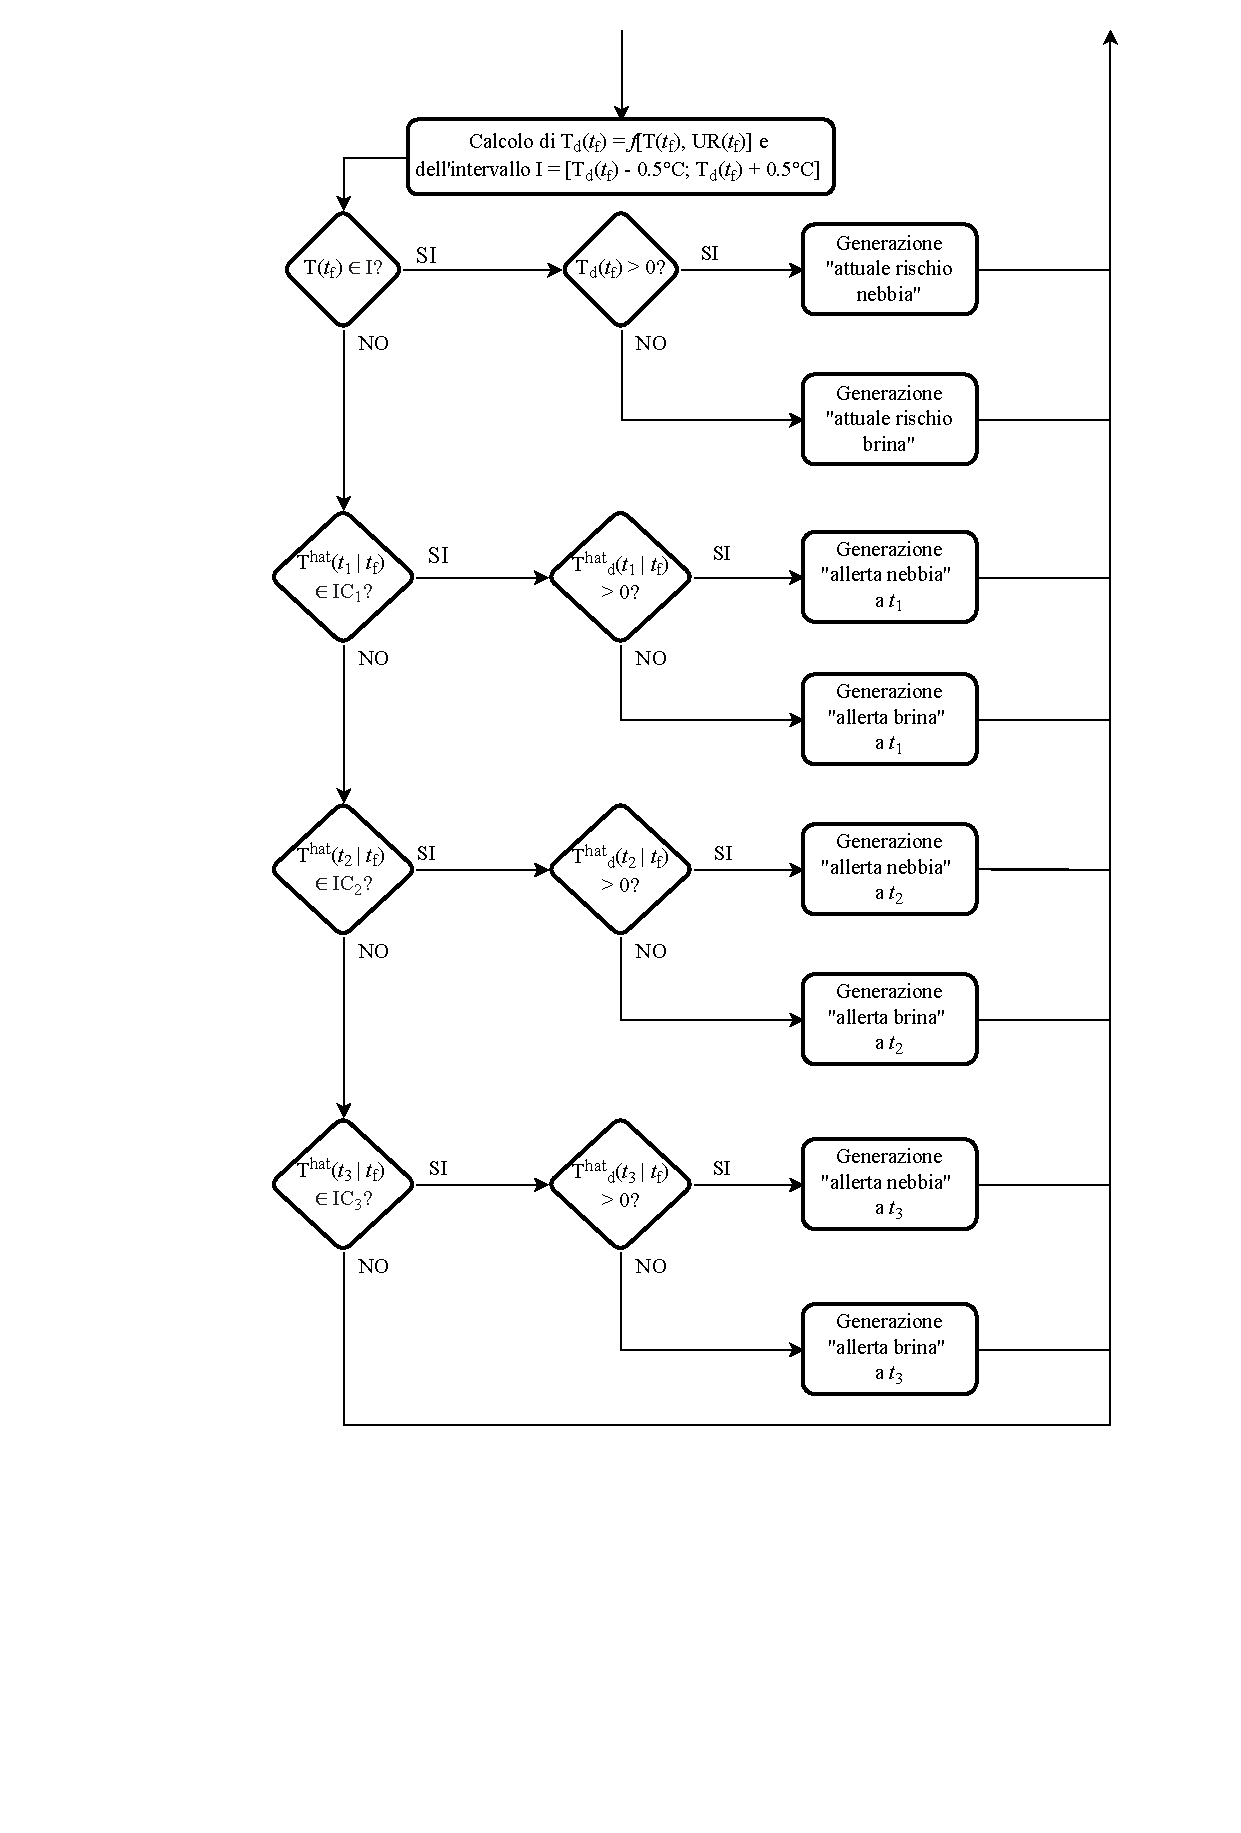
\includegraphics[height=580px]{FlowChartsFiles/Allerte_nebbia_&_brina_2.pdf}
	\caption[Diagramma di flusso relativo al processo di generazione di allerte nebbia e brina (2)]{diagramma di flusso relativo al processo di generazione di allerte nebbia e brina (2).}
	\label{Allerta_nebbia_&_brina_2}
\end{figure}

